% Options for packages loaded elsewhere
\PassOptionsToPackage{unicode}{hyperref}
\PassOptionsToPackage{hyphens}{url}
\PassOptionsToPackage{dvipsnames,svgnames,x11names}{xcolor}
%
\documentclass[
  12pt]{article}

\usepackage{amsmath,amssymb}
\usepackage{iftex}
\ifPDFTeX
  \usepackage[T1]{fontenc}
  \usepackage[utf8]{inputenc}
  \usepackage{textcomp} % provide euro and other symbols
\else % if luatex or xetex
  \usepackage{unicode-math}
  \defaultfontfeatures{Scale=MatchLowercase}
  \defaultfontfeatures[\rmfamily]{Ligatures=TeX,Scale=1}
\fi
\usepackage{lmodern}
\ifPDFTeX\else  
    % xetex/luatex font selection
\fi
% Use upquote if available, for straight quotes in verbatim environments
\IfFileExists{upquote.sty}{\usepackage{upquote}}{}
\IfFileExists{microtype.sty}{% use microtype if available
  \usepackage[]{microtype}
  \UseMicrotypeSet[protrusion]{basicmath} % disable protrusion for tt fonts
}{}
\makeatletter
\@ifundefined{KOMAClassName}{% if non-KOMA class
  \IfFileExists{parskip.sty}{%
    \usepackage{parskip}
  }{% else
    \setlength{\parindent}{0pt}
    \setlength{\parskip}{6pt plus 2pt minus 1pt}}
}{% if KOMA class
  \KOMAoptions{parskip=half}}
\makeatother
\usepackage{xcolor}
\setlength{\emergencystretch}{3em} % prevent overfull lines
\setcounter{secnumdepth}{5}
% Make \paragraph and \subparagraph free-standing
\ifx\paragraph\undefined\else
  \let\oldparagraph\paragraph
  \renewcommand{\paragraph}[1]{\oldparagraph{#1}\mbox{}}
\fi
\ifx\subparagraph\undefined\else
  \let\oldsubparagraph\subparagraph
  \renewcommand{\subparagraph}[1]{\oldsubparagraph{#1}\mbox{}}
\fi


\providecommand{\tightlist}{%
  \setlength{\itemsep}{0pt}\setlength{\parskip}{0pt}}\usepackage{longtable,booktabs,array}
\usepackage{calc} % for calculating minipage widths
% Correct order of tables after \paragraph or \subparagraph
\usepackage{etoolbox}
\makeatletter
\patchcmd\longtable{\par}{\if@noskipsec\mbox{}\fi\par}{}{}
\makeatother
% Allow footnotes in longtable head/foot
\IfFileExists{footnotehyper.sty}{\usepackage{footnotehyper}}{\usepackage{footnote}}
\makesavenoteenv{longtable}
\usepackage{graphicx}
\makeatletter
\def\maxwidth{\ifdim\Gin@nat@width>\linewidth\linewidth\else\Gin@nat@width\fi}
\def\maxheight{\ifdim\Gin@nat@height>\textheight\textheight\else\Gin@nat@height\fi}
\makeatother
% Scale images if necessary, so that they will not overflow the page
% margins by default, and it is still possible to overwrite the defaults
% using explicit options in \includegraphics[width, height, ...]{}
\setkeys{Gin}{width=\maxwidth,height=\maxheight,keepaspectratio}
% Set default figure placement to htbp
\makeatletter
\def\fps@figure{htbp}
\makeatother

\addtolength{\oddsidemargin}{-.5in}%
\addtolength{\evensidemargin}{-1in}%
\addtolength{\textwidth}{1in}%
\addtolength{\textheight}{1.7in}%
\addtolength{\topmargin}{-1in}%
\makeatletter
\makeatother
\makeatletter
\makeatother
\makeatletter
\@ifpackageloaded{caption}{}{\usepackage{caption}}
\AtBeginDocument{%
\ifdefined\contentsname
  \renewcommand*\contentsname{Table of contents}
\else
  \newcommand\contentsname{Table of contents}
\fi
\ifdefined\listfigurename
  \renewcommand*\listfigurename{List of Figures}
\else
  \newcommand\listfigurename{List of Figures}
\fi
\ifdefined\listtablename
  \renewcommand*\listtablename{List of Tables}
\else
  \newcommand\listtablename{List of Tables}
\fi
\ifdefined\figurename
  \renewcommand*\figurename{Figure}
\else
  \newcommand\figurename{Figure}
\fi
\ifdefined\tablename
  \renewcommand*\tablename{Table}
\else
  \newcommand\tablename{Table}
\fi
}
\@ifpackageloaded{float}{}{\usepackage{float}}
\floatstyle{ruled}
\@ifundefined{c@chapter}{\newfloat{codelisting}{h}{lop}}{\newfloat{codelisting}{h}{lop}[chapter]}
\floatname{codelisting}{Listing}
\newcommand*\listoflistings{\listof{codelisting}{List of Listings}}
\makeatother
\makeatletter
\@ifpackageloaded{caption}{}{\usepackage{caption}}
\@ifpackageloaded{subcaption}{}{\usepackage{subcaption}}
\makeatother
\makeatletter
\@ifpackageloaded{tcolorbox}{}{\usepackage[skins,breakable]{tcolorbox}}
\makeatother
\makeatletter
\@ifundefined{shadecolor}{\definecolor{shadecolor}{rgb}{.97, .97, .97}}
\makeatother
\makeatletter
\makeatother
\makeatletter
\makeatother
\ifLuaTeX
  \usepackage{selnolig}  % disable illegal ligatures
\fi
\usepackage[]{natbib}
\bibliographystyle{agsm}
\IfFileExists{bookmark.sty}{\usepackage{bookmark}}{\usepackage{hyperref}}
\IfFileExists{xurl.sty}{\usepackage{xurl}}{} % add URL line breaks if available
\urlstyle{same} % disable monospaced font for URLs
\hypersetup{
  pdftitle={Debt Ceiling Brinkmanship and Global Financial Diversification},
  pdfauthor={William Clinton Co},
  pdfkeywords={3 to 6 keywords, that do not appear in the title},
  colorlinks=true,
  linkcolor={blue},
  filecolor={Maroon},
  citecolor={Blue},
  urlcolor={Blue},
  pdfcreator={LaTeX via pandoc}}


\begin{document}


\def\spacingset#1{\renewcommand{\baselinestretch}%
{#1}\small\normalsize} \spacingset{1}


%%%%%%%%%%%%%%%%%%%%%%%%%%%%%%%%%%%%%%%%%%%%%%%%%%%%%%%%%%%%%%%%%%%%%%%%%%%%%%

\date{June 30, 2023}
\title{\bf Debt Ceiling Brinkmanship and Global Financial
Diversification}
\author{
William Clinton Co\thanks{Below is an attached research proposal. It
starts with an introduction. Followed by relevant data sets along with
proposed methodology. Lastly, a game theory model of debt ceiling
brinkmanship is proposed.}\\
Department of Economics, The University of British Columbia\\
}
\maketitle

\bigskip
\bigskip
\begin{abstract}
The text of your abstract. 200 or fewer words.
\end{abstract}

\noindent%
{\it Keywords:} 3 to 6 keywords, that do not appear in the title
\vfill

\newpage
\spacingset{1.9} % DON'T change the spacing!
\ifdefined\Shaded\renewenvironment{Shaded}{\begin{tcolorbox}[interior hidden, frame hidden, boxrule=0pt, borderline west={3pt}{0pt}{shadecolor}, breakable, enhanced, sharp corners]}{\end{tcolorbox}}\fi

\hypertarget{sec-intro}{%
\section{Introduction}\label{sec-intro}}

Constantly increasing public debt has been a recent occurrence
throughout recent history \citet{mitchener2023}. This raises the
question of how will governments deal with rising debt burdens going
forward. As debt increases, cost of borrowing increases. Do governments
internalize the increase of cost of borrowing, in the context of debt
ceiling brinkmanship? We construct a data set of X-dates, dates where
the US government will supposedly run out of money. We then analyze the
CDS prices and yield spreads, such that we investigate weather debt
ceiling negotiations will settle earlier given a bigger increased in
cost of capital.We investigate trends overtime.

It has also been noted we have debt crisis without default has become
more common, wherein there was a near missed payment but never a default
has a negative effect on output, as exemplified in Greece Portugal and
Spain during 2010-2012 \citet{mitchener2023} . Going a step further some
have propose to change the definition of debt crises to yield spreads of
1000 basis points, also known as spread spikes.
\citep{broner2013, aguiar, krishnamurthy}

There has been work on the frequency of debt crisis without default. we
study this data set by cite \citet{meyer2022} as it relates data on debt
ceiling brinkmanship \citet{reinhart2008} we use the defintion of 1000
basis points we analyze these in the context of debt brinkmanship taking
inspiration from graphs.

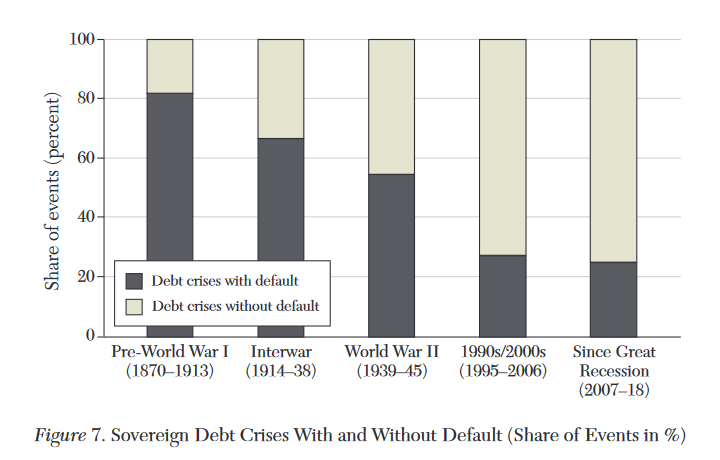
\includegraphics{style-guide/overtime_brink_1.png}

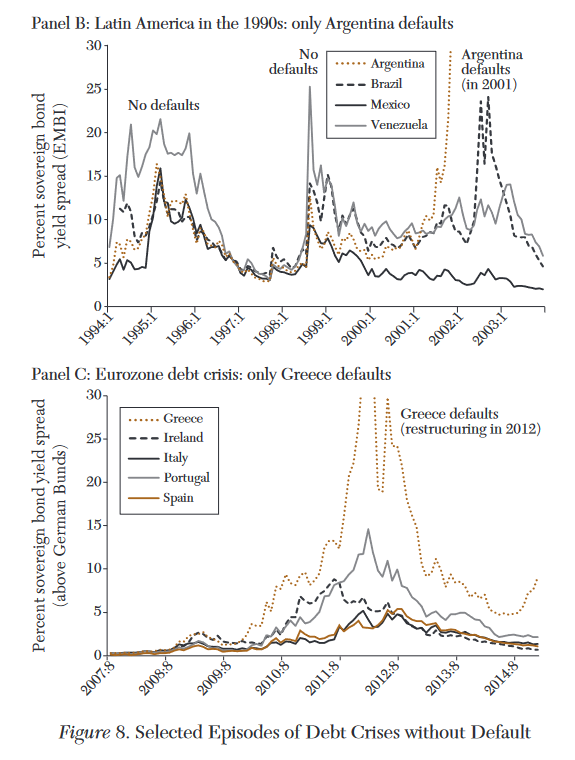
\includegraphics{style-guide/overtime_brink_2.png}

What makes this even more poignant is that the output decline happens in
anticipation of a default rather than the default itself
\citet{yeyati2011} . Thus we investigate if this link applies to debt
ceiling brinkmanship as well.

What makes this an important topic to study is the body of evidence
proving a decline in output associated with the high yields that
accompanies a debt crisis. There are varying reasons for this such as
the relationship between external financing and importers
\citet{mendoza2012} , the decrease in external domestic firm
borrowing\citep{corsetti2012, das2010, gourinchas2016} or the tightening
of credit against loses on bank balance
sheets\citep{arellano, ferrando2017}.Similarly, we explore this in the
context of debt brinkmanship.

There has also been work on how credit rating agencies downgrading
reduces leverage and investments \citet{almeida2017}. Similar
conclusions were drawn using CDS premia instead of bond yield spreads
\citep{brutti2015, bahaj2020}. Similarly, we explore this in the context
of debt brinkmanship.

Another pertinent question is the many creditors willing to lend to
highly indebted sovereigns. Currently we are in a safe asset shortage,
such that we are coming closer to the effective lower bound, wherein
central banks could not decrease interest rates any further as needed.
This shortage is a key source of fragility in the economy, dubbed the
``safety trap''. \citet{caballero2017We} investigate if brinkmanship is
a contributor to the shortage of safe assets. If so then there would be
an argument to abolish the system on a global welfare standpoint. Taking
inspiration from

track how china plays into this . Track Chinese investments.

advanced vs developed

Track advance vs developed economies effects

currency composition-\/- world currency composition. I track the
investment. I track the currencies.

\begin{figure}

{\centering 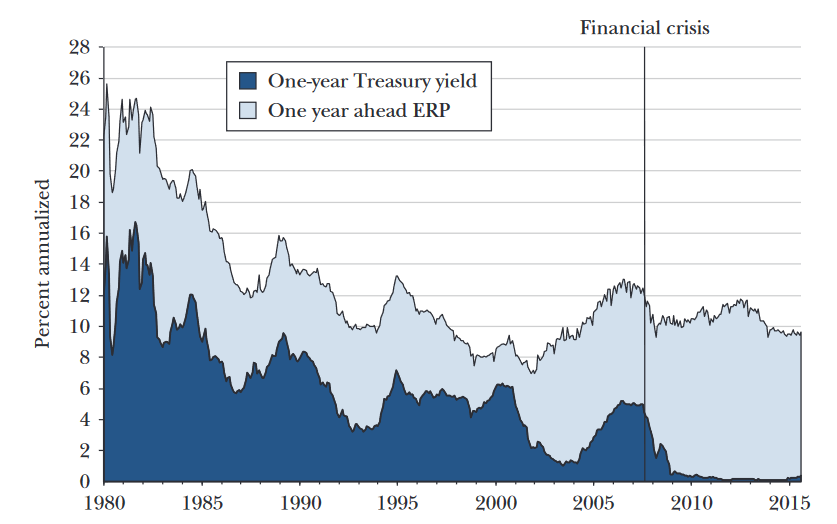
\includegraphics{style-guide/1_year_ERP.png}

}

\caption{\label{fig-first}Consistency comparison in fitting surrogate
model in the tidal power example.}

\end{figure}

We use the 1 year expected risk premium vs the 1 year treasury yield to
construct a similar graph that marks debt ceiling brinkmanship.
Furthermore we construct the graph below with the same variables
\citet{duarte2015}.

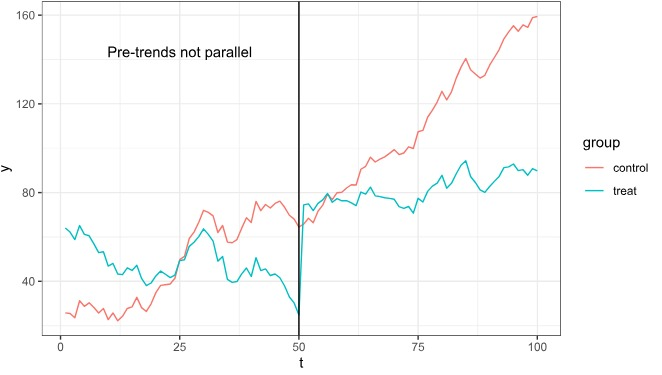
\includegraphics{style-guide/1_year_ERP_parallel_trends.jpeg}

given the outsize buying of central banks we look at

. By answering this question we gain insight into the future of larger
and larger public debt burdens going forward.

We investigate if its ias a threat to safe asset shortage.

The US treasury yield occupies the status as the biggest and most liquid
market, wherein its yield is a signicant determinant of the global
factor of yields.

Given that the global factor has become increasingly a more important
determinant of yields ,against the specific ``country'' factor
\citet{mauro2002}. thus it becomes important to study this
phenomenon.\citep{rozada2006, gonzález-rozada2008, longstaff2011}

\hypertarget{sec-dataset}{%
\section{Data set}\label{sec-dataset}}


\renewcommand\refname{References}
  \bibliography{bibliography.bib}


\end{document}
